\section{Introduction to Schumacher's Compression Theorem}

\begin{frame}{Shannon's Source Coding Theorem}
    \textbf{Classical Context:} Shannon's theorem provides the foundation for lossless data compression:
    \begin{itemize}
        \item It ensures data can be encoded efficiently without losing information.
        \item In the limit of long sequences, the average number of bits required per symbol equals the entropy of the source \( H(X) \).
    \end{itemize}
    \textbf{Formula:}
    \[
    H(X) = -\sum_{x \in \mathcal{X}} P(x) \log_2 P(x),
    \]
    where \( P(x) \) is the probability of symbol \( x \).
    \begin{figure}[h]
        \centering
        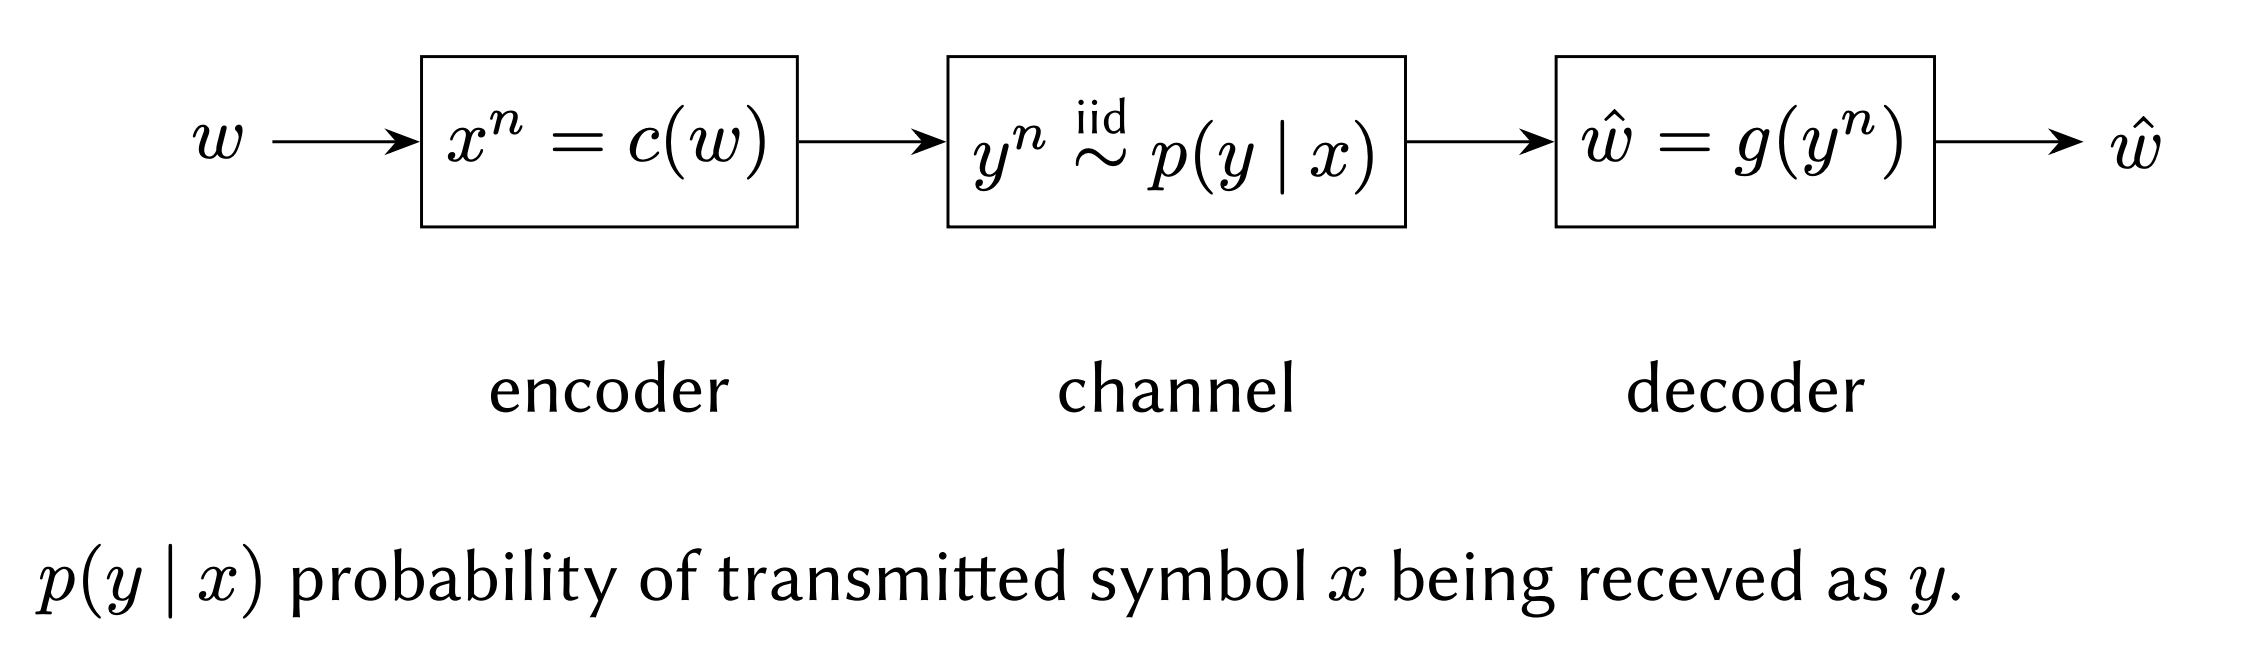
\includegraphics[width=0.75\textwidth]{figures/shannon_pic.png}
        \caption{Shannon's Noisy Channel Theorem \cite{jahooShannonsNoisy}}
    \end{figure}
\end{frame}

\begin{frame}{Schumacher's Compression Theorem}
    Schumacher's theorem extends Shannon's ideas to quantum systems, enabling lossless compression of quantum states.
    \begin{block}{Key Idea}
        \begin{itemize}
            \item Use \textbf{qubits}, the fundamental units of quantum information.
            \item Compress \( n \)-copy quantum states described by a density matrix \( \rho \) to occupy a subspace of dimension \( 2^{n S(\rho)} \), where \( S(\rho) \) is the von Neumann entropy.
        \end{itemize}
    \end{block}
    \textbf{Theorem Statement:}
    \begin{enumerate}
        \item For a source emitting states described by \( \rho \), the minimum qubits needed for \( n \) copies is \( n S(\rho) \).
        \item The data can be compressed with nearly perfect fidelity as \( n \to \infty \).
    \end{enumerate}
    \begin{figure}[h]
        \centering
        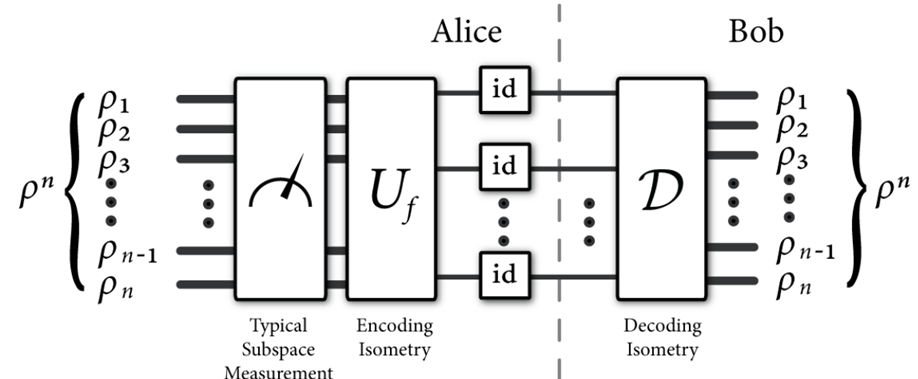
\includegraphics[width=0.75\textwidth]{figures/schumacher.png}
        \caption{Schumacher Info Picture \cite{PhysRevA.51.2738}}
    \end{figure}
\end{frame}

\section{Key Concepts in Schumacher's Theorem}

\begin{frame}{Quantum States and Density Matrices}
    \begin{itemize}
        \item A quantum state is described by a density matrix \( \rho \), particularly for mixed states.
        \item If a source emits states \( \{ |\psi_i\rangle \} \) with probabilities \( \{ p_i \} \), the density matrix is:
        \[
        \rho = \sum_i p_i |\psi_i\rangle \langle \psi_i|.
        \]
        \item The von Neumann entropy \( S(\rho) \) measures the quantum uncertainty:
        \[
        S(\rho) = -\text{Tr}(\rho \log \rho).
        \]
    \end{itemize}
\end{frame}

\begin{frame}{Typical Subspaces}
    \textbf{Key Concept:} The typical subspace captures the most probable sequences emitted by a quantum source.
    \begin{block}{Definition}
        An \(\epsilon\)-typical sequence \((i_1, i_2, \dots, i_n)\) satisfies:
        \[
        \left| -\frac{1}{n} \log p_{i_1 i_2 \dots i_n} - S(\rho) \right| < \epsilon,
        \]
        where \( p_{i_1 i_2 \dots i_n} = p_{i_1} p_{i_2} \cdots p_{i_n} \).
    \end{block}
    \textbf{Properties:}
    \begin{itemize}
        \item High probability: Most of the probability mass lies in the typical subspace.
        \item Dimension: 
        \[
        2^{n(S(\rho) - \epsilon)} \leq \dim(\mathcal{H}_{\text{typ}}) \leq 2^{n(S(\rho) + \epsilon)}.
        \]
    \end{itemize}
\end{frame}

% Section: Proof of Schumacher's Theorem
\section{Proof of Schumacher's Theorem}

\begin{frame}{Proof of Achievability}
    \textbf{Goal:} Achieve asymptotically perfect fidelity for \( R > S(\rho) \).
    \begin{enumerate}
        \item \textbf{Projector Construction:}
        \[
        \Pi_{n, \epsilon} = \sum_{(i_1, \dots, i_n) \in T_{n, \epsilon}} |\psi_{i_1} \otimes \cdots \otimes \psi_{i_n}\rangle \langle \psi_{i_1} \otimes \cdots \otimes \psi_{i_n}|.
        \]
        \item \textbf{Encoding Channel:} Map states into the typical subspace:
        \[
        E_n(\rho^{\otimes n}) = 
        \begin{cases}
            V_{n, \epsilon} \rho^{\otimes n} V_{n, \epsilon}^\dagger, & \text{if } \rho^{\otimes n} \in \mathcal{H}_{\text{typ}}; \\
            |0\rangle\langle 0|, & \text{otherwise.}
        \end{cases}
        \]
        \item \textbf{Decoding Channel:} Recover states from the typical subspace:
        \[
        D_n(Y) = V_{n, \epsilon}^\dagger Y V_{n, \epsilon}.
        \]
    \end{enumerate}
\end{frame}

\begin{frame}{Fidelity}
    The fidelity between the original state and the reconstructed state satisfies:
    \[
    F(D_n \circ E_n, \rho^{\otimes n}) \geq \text{Tr}[\Pi_{n, \epsilon} \rho^{\otimes n}] \to 1 \quad \text{as } n \to \infty.
    \]
    \textbf{Achievable Compression Rate:}
    \begin{itemize}
        \item Number of qubits required: \( m_n = \lceil \log_2 \dim(\mathcal{H}_{\text{typ}}) \rceil \).
        \item Compression rate:
        \[
        R = \lim_{n \to \infty} \frac{m_n}{n} \leq S(\rho) + \epsilon.
        \]
        \item For \( R > S(\rho) \), choose \( \epsilon > 0 \) sufficiently small to achieve high fidelity.
    \end{itemize}
\end{frame}

\begin{frame}{Proof of Converse}
    \textbf{Goal:} Show that \( R < S(\rho) \) results in fidelity \( \to 0 \).
    \begin{block}{Key Idea}
        \begin{itemize}
            \item The compressed space \( \dim = 2^{n_k R} \) is exponentially smaller than the typical subspace \( \dim = 2^{n_k S(\rho)} \).
            \item Kraus decomposition bounds fidelity:
            \[
            F(D_k \circ E_k, \rho^{\otimes n_k}) \leq \sqrt{\sum_{l=1}^{L_k} q_l \cdot \text{Tr}[\Pi_l \rho^{\otimes n_k}]}.
            \]
        \end{itemize}
    \end{block}
    Since \( R < S(\rho) \), it follows:
    \[
    \text{Tr}[\Pi_l \rho^{\otimes n_k}] \to 0 \quad \implies \quad F(D_k \circ E_k, \rho^{\otimes n_k}) \to 0.
    \]
\end{frame}

\section{Image Citations}

\begin{figure}[h]
    \centering
    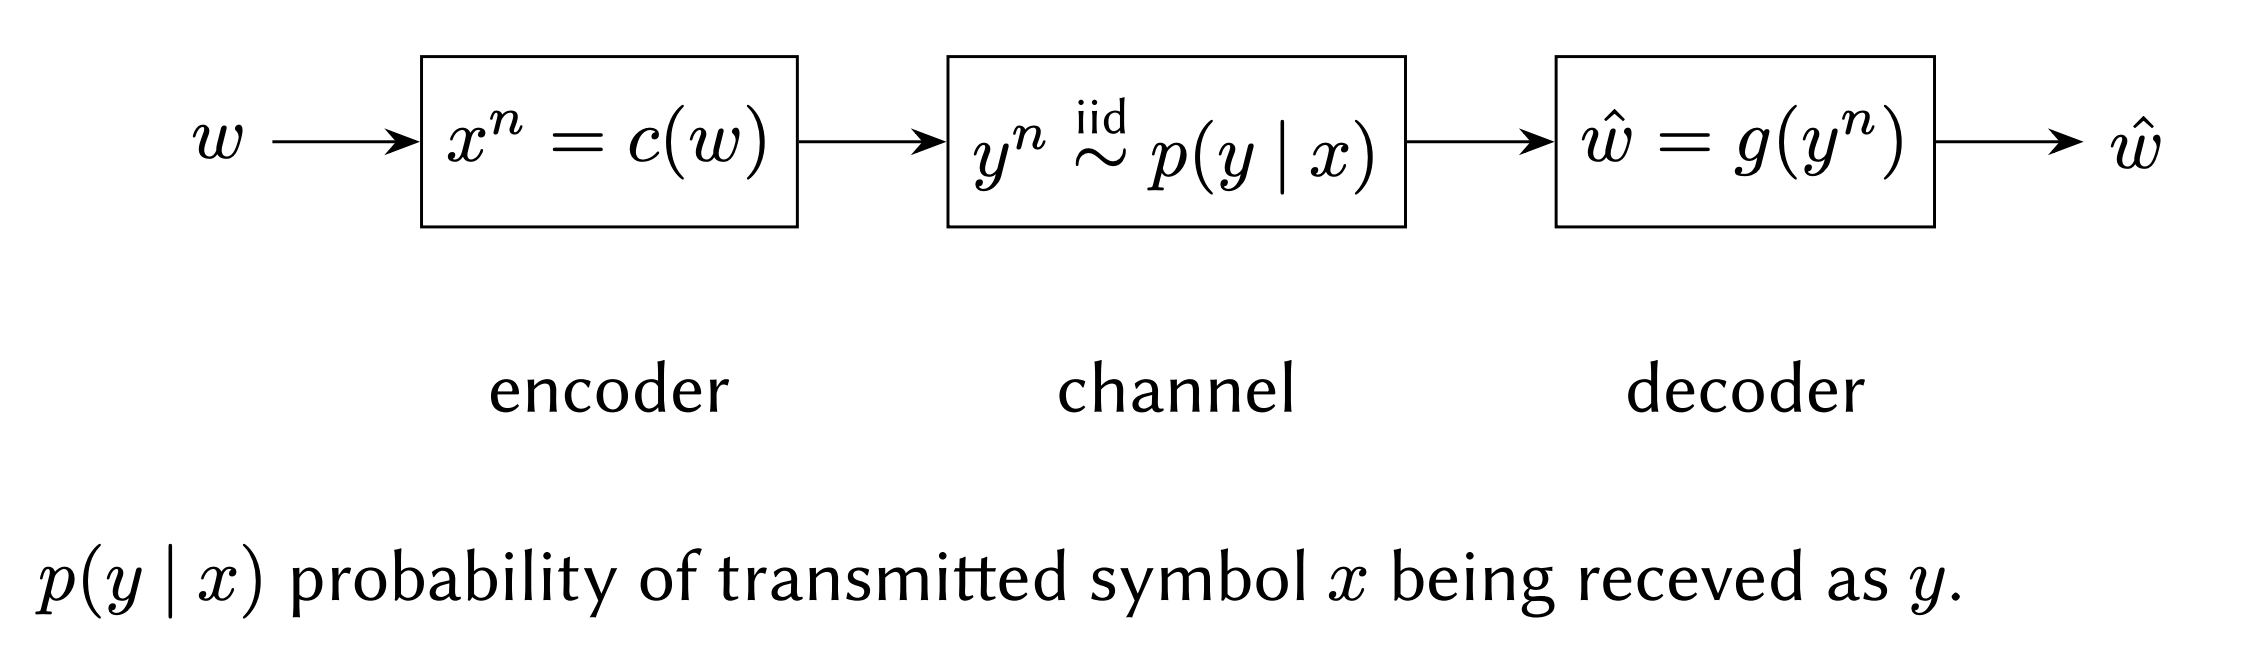
\includegraphics[width=0.75\textwidth]{figures/shannon_pic.png}
    \caption{Shannon's Noisy Channel Theorem \cite{jahooShannonsNoisy}}
\end{figure}

\begin{figure}[h]
    \centering
    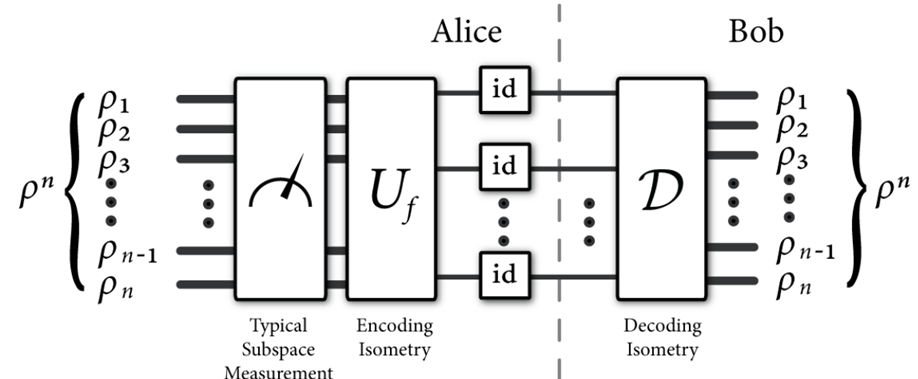
\includegraphics[width=0.75\textwidth]{figures/schumacher.png}
    \caption{Schumacher Info Picture \cite{PhysRevA.51.2738}}
\end{figure}
